% \documentclass[handout]{beamer} % use this for handouts
\documentclass{beamer}
\usepackage{codestyle}
\usepackage{pagestyle}
\usetheme{Copenhagen}
% make the header more minimal 
\setbeamertemplate{headline}{
    \leavevmode
    \hbox{%
        \begin{beamercolorbox}[wd=\paperwidth,ht=2.5ex,dp=1.125ex]{section in head/foot}%
            \insertsectionnavigationhorizontal{\paperwidth}{}{}
        \end{beamercolorbox}%
    }
}

% remove the footer in the copenhagen theme
\setbeamertemplate{footline}{}

\title{Cross-Language Component Testing: Performance and Interoperability Insights}
\author{Kai Erik Niermann}
\date{\today}

\begin{document}

\frame{\titlepage}

\begin{frame}
\frametitle{Outline}
\tableofcontents
\end{frame}

\section{Introduction}
\begin{frame}{Introduction}
    \begin{itemize}
        \item Establishing terminology
        \pause
        \item \textbf{Rewrite}:
        \begin{itemize}
            \item Writing new code
            \item Same or new language
            \item Implements existing features
        \end{itemize}
        \pause
        \item \textbf{Refactoring}:
        \begin{itemize}
            \item Rearrange/minimize existing code
        \end{itemize}
        \pause
        \item Reasons for rewrites:
        \begin{itemize}
            \item Second system effect
            \item New developments in libraries/languages
            \item Initial choices restrictive as application scales
        \end{itemize}
        \pause
        \item Benefits and drawbacks:
        \begin{itemize}
            \item Overimplementation risk (Fred Brooks)
            \item Better understanding and new technologies
        \end{itemize}
        \pause
        \item Rewrites in software development:
        \begin{itemize}
            \item Key component
            \item Thesis explores effective approaches
        \end{itemize}
    \end{itemize}
\end{frame}
\subsection{Motivation}
\begin{frame}{Motivation}
    \textbf{Definition}
    \begin{itemize}
        \item Using a different language for rewriting existing code
    \end{itemize}
    \pause
    \textbf{Benefits}
    \begin{itemize}
        \item Addresses fundamental limitations of the original language
    \end{itemize}
    \pause
    \textbf{Challenges}
    \begin{itemize}
        \item Effectiveness of new language
        \item Large system size
        \item Unforeseen incompatibilities
    \end{itemize}
    \pause
    \textbf{Testing Approach}
    \begin{itemize}
        \item Test a critical component first
        \item Minimal additional code
    \end{itemize}
    \pause
    \textbf{Strategies}
    \begin{itemize}
        \item Wrap component in testing framework
        \item Use language interop APIs
    \end{itemize}
    \pause
    \textbf{Objective}
    \begin{itemize}
        \item Determine if the component works better in another language
    \end{itemize}
\end{frame} 

\section{Research Questions}

\begin{frame}{Research Questions}
    \begin{block}{Main Question}
        How can we test the performance of a system component rewritten in another programming language?
    \end{block}

    \pause

    \begin{block}{Role of Language APIs}
        How do language APIs differ in their approaches to mapping objects and types, are some more restrictive than others?
    \end{block}

    \pause

    \begin{block}{Performance and Real world applications}
        How does the overhead and restrictions on optimization techniques effect their application in performance performance dependent production code?
    \end{block}

\end{frame}

\section{Study design}
\subsection{System Design}
\begin{frame}{system design}
    \begin{columns}
        \begin{column}{0.5\textwidth}
            \begin{figure}
                \centering
                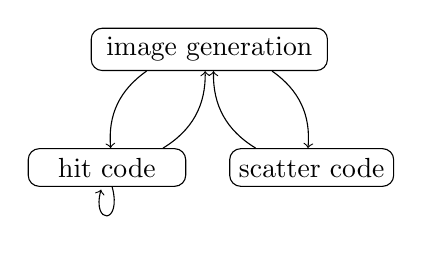
\begin{tikzpicture}[->]
                    \node[draw, rectangle, rounded corners, minimum width=3cm] (A) at (0, 0) {image generation};
                    \node[draw, rectangle, rounded corners, minimum width=2cm] (B) at (-1.3, -1.5) {hit code};
                    \node[draw, rectangle, rounded corners, minimum width=2cm] (C) at (1.3, -1.5) {scatter code};
                    
                    \draw (A) edge[bend right] (B);
                    \draw (B) edge[bend right] (A);

                    \draw (A) edge[bend left] (C);
                    \draw (C) edge[bend left] (A);
                    
                    \path (B) edge [loop below] (B);
                \end{tikzpicture}
                \caption{Ray tracer overview }
            \end{figure}
        \end{column}
        \pause
        \begin{column}{0.5\textwidth}
            \begin{itemize}
                \item Complex enough system to demonstrate the idea in an applied setting.
                \pause 
                \item Distinct components that can be isolated for testing.
                \pause 
                \item Requires high performance to function effectively, making it ideal for assessing performance needs.
            \end{itemize}
        \end{column}
    \end{columns}
\end{frame}
\subsection{Approach}
\begin{frame}{Testing Approach: Q \& A Format}
    \begin{itemize}
        \item How do we isolate the most performance impacting component?
        \begin{itemize}
            \item Profile our application for runtime and memory.
            \item Use the profiling data to make a judgement on the most performance impacting component.
        \end{itemize}
        \pause
        \item What languages do we choose for rewriting?
        \begin{itemize}
            \item Choose languages with embedding APIs for Julia. 
            \item Opt for Python and C++ due to their differing fundamental properties and available interface libraries.
        \end{itemize}
        \pause
        \item How do we test the rewritten components?
        \begin{itemize}
            \item Use the language specific benchmarking tools to test components in isolation.
            \item Use Julia's benchmarking tools to test compontents \& overhead 
        \end{itemize}
    \end{itemize}
\end{frame}

\section{Methodology}
\subsection{rewriting}
\input{rewriting.tex}
\subsection{choice of apis}

\begin{frame}
    \frametitle{Choosing an Interop API}
    
    Choosing the right embedding API to attach hit functions to the ray tracer implementation was crucial.
    
    \pause
    
    \textbf{Python}
    \begin{itemize}
        \item Python/JuliaCall API:
        \begin{itemize}
            \item Builds on previous implementations.
            \item Supports extensive language conversions.
        \end{itemize}
    \end{itemize}
    
    \pause
    
    \textbf{C++}
    \begin{itemize}
        \item Options:
        \begin{itemize}
            \item CxxWrap: Feature-rich but less user-friendly.
            \item (\textbf{choice}) Jluna: Newer, user-friendly, lacks some features
        \end{itemize}
    \end{itemize}
    
    \pause
    
    \textbf{Considerations}
    \begin{enumerate}
        \item Choose an API that minimizes additional code.
        \item Prefer an API that simplifies component attachment.
    \end{enumerate}
    
    \pause
    
    Languages supporting reflection reduce additional code, simplifying rewriting and testing.
    
    \end{frame}
\subsection{testing setup}
\input{testing-setup.tex}

\subsection{mapping}

\begin{frame}{Mapping Objects to Statically Typed Languages}
    \textbf{Static Mapping}
    \begin{itemize}
        \item User describes interface for types (e.g., class/struct).
        \item API maps Julia type to corresponding C++ type.
        \item User-defined reflection system parses low-level types.
    \end{itemize}
    
    \vspace{0.5cm}
    \pause
    \textbf{Getters and Setters:}
    \begin{itemize}
        \item Define functions $\text{get}(x)$ and $\text{put}(x)$.
        \item Property $x$ represented as a string.
        \item $\text{get}: S \rightarrow V = \text{object property } x$
        \item $\text{set}: S, V \rightarrow S = \text{modified property } x$
    \end{itemize}
    
    \vspace{0.5cm}
    \pause
    \textbf{Note:} Similar to functional programming lens.
\end{frame}
\begin{frame}{Challenges with Getter/Setter Pairs}
    \begin{block}{Limitation} 
        Issues arise when source $S$ has an abstract type.
    \end{block}
    \textbf{Notation}
        \begin{itemize}
            \item $[S: T]$, $[V: T]$ represent source and value types.
            \item $\text{set}: [S: T_B], [V: T_{bi}] \rightarrow S_m$
        \end{itemize}
    \textit{Problem}: Julia uses strings for type representation:
        \begin{itemize}
            \item $\text{set}: [S: T_B], [V: \text{str}(T_{bi})] \rightarrow S_m$
            \item Need to map strings to C++ types.
        \end{itemize}
    \textit{Solution}: Create a mapping mechanism
        \begin{itemize}
            \item string to type mapping $st$ and type comparison $f$:
            \[
                st: \text{str}(T_i) \rightarrow \text{typeinf}(T_i) \quad f: st, \text{typeinf}(T_p) \rightarrow \text{bool}
            \]
            \item Use compile-time code generation with variadic templates.
        \end{itemize}
    Achieve correspondence using fold expressions on variadic templates.
\end{frame}
\subsection{improved static mapping}
\begin{frame}
    \frametitle{Optimizing Setter Functions}
    
    Key issue with trivial approach
    \begin{itemize}
      \item Requires providing all derived types to each getter/setter pair.
      \item Leads to annoying repeated user defined code and potential errors.
    \end{itemize}
    \pause 
    \textit{Preferable solution}
    \begin{itemize}
      \item Define the set of derived types once.
      \item Allow all setters for attributes of a class to access this information.
    \end{itemize}
\end{frame}
\input{no-reflect-better3.tex}

\section{Discussion}
\begin{frame}{Limitations}
    \textbf{Considerations}
    \begin{itemize}
        \item Users must specify class properties via lambdas. 
        \begin{itemize}
            \item Macros can simplify this process but its not ideal.
        \end{itemize}
        \pause
        \item All derived types must be passed to objects with base type attributes.
        \begin{itemize}
            \item Tradeoff in library complexity and maintainability vs user defined types. 
        \end{itemize} 
        \pause
        \item Still requires additional user defined type specifications to allow for introspection
    \end{itemize}
    \pause
    \begin{block}{key challenge}
        Find some means of having the base type interface discern the correct derived type to instantiate.
    \end{block}
\end{frame}
    
\begin{frame}
    \frametitle{Benefits}
    
    This system offers
    \begin{itemize}
      \item Simplified object deduction process
      \item Ability to map abstract objects
      \item Utilization of modern C++ principles for futureproofing
      \item Increased maintainability and extensibility
      \item Possiblity to adapt this when Reflection TS becomes available in C++26
    \end{itemize}
    \pause
    \begin{block}{Key Takeaway}
        It provides a more concise approach compared to traditional methods, enhancing ease of implementation and potential for future extensions.
    \end{block}
\end{frame}
\begin{frame}{Insights}
    
    \textbf{Observations}
    \begin{itemize}
      \item Possible to implement a generic method for polymorphic object mapping.
      \item Offers JuliaCall API capabilities with C++ speed.
      \item Requires Julia data copying due to Julia C API limitations.
    \end{itemize}
    \pause
    \textbf{Main takeaways}
    \begin{itemize}
      \item Metaprogramming approaches effective for object reflection
      \item We can map to static languages with minimal additional boilerplate
      \item Straightforward testing and integration across languages
    \end{itemize}
    \end{frame}
    
\section{Results}
\begin{frame}{Baseline performance}
\end{frame}
\begin{frame}{Isolated Performance - RQ3}
        \textbf{Results}
        \begin{itemize}
            \item C++ outperforms Julia and Python in component runtime.
            \item Substantial overhead from Julia API (dynamic dispatch, type inference).
            \item Julia performs well with type stability, hindered by cross-language calls.
        \end{itemize}
        \pause
        \textbf{Conclusion}
        \begin{itemize}
            \item High-performance interop between different languages is challenging.
            \item Effective on a smaller scale, but less viable for very different languages.
        \end{itemize}
    \begin{center}
        \includegraphics[width=0.45\textwidth]{assets/time-and-overhead-log.png} % Replace with your actual diagram file
    \end{center}
\end{frame}
\begin{frame}{Results and Takeaways}
    \begin{itemize}
        \item Different language APIs have varied integration approaches.
        \item Adapting APIs to specific use cases is generally manageable depending on the language
        \item Metaprogramming is effective for implementing generic, extensible interop libraries.
        \item Performance overhead mainly due to language incompatibilities.
        \item Mitigation possible with languages using similar execution methods.
        \item APIs work well for testing components.
        \item Careful consideration needed for using these APIs in performance-dependent production code.
    \end{itemize}
\end{frame}

\end{document}
